%%==========================================================================
%% This is the very first version of a Streetwise LaTeX template. By
%% chosing the document class, it is easily convertible to a two-column IEEE
%% paper format, provided any conflicting packages and (new)commmands are
%% removed.
%%
%% Erwin de Gelder, January 6, 2018
%%==========================================================================

%%==========================================================================
%% Title:
%% Author(s):
%% To be published in:
%% Date of submission:
%% Date of submission R1:
%% Date of submission R2:
%% Date of final submission:
%%==========================================================================


%% Generic
\documentclass[10pt,final,a4paper,oneside,onecolumn]{article}

%% IEEE
%% Document class options: replace "draftcls" by "final" for final document.
%% All other options may just as well be omitted because they are the default values.
%\documentclass[10pt,final,journal,letterpaper,twoside,twocolumn]{IEEEtran}


%%==========================================================================
%% Document automation
%%==========================================================================

\def\reptitle{Ontology for traffic scenarios}
\def\repauthor{Erwin de Gelder, etc.}


%%==========================================================================
%% Packages
%%==========================================================================

\usepackage[a4paper,left=3.5cm,right=3.5cm,top=3cm,bottom=3cm]{geometry} %% change page layout; remove for IEEE paper format
\usepackage[T1]{fontenc}                        %% output font encoding for international characters (e.g., accented)
\usepackage[cmex10]{amsmath}                    %% math typesetting; consider using the [cmex10] option
\usepackage{amssymb}                            %% special (symbol) fonts for math typesetting
\usepackage{amsthm}                             %% theorem styles
\usepackage{dsfont}                             %% double stroke roman fonts: the real numbers R: $\mathds{R}$
\usepackage{mathrsfs}                           %% formal script fonts: the Laplace transform L: $\mathscr{L}$
\usepackage[pdftex]{graphicx}                   %% graphics control; use dvips for TeXify; use pdftex for PDFTeXify
\usepackage{array}                              %% array functionality (array, tabular)
\usepackage{upgreek}                            %% upright Greek letters; add the prefix 'up', e.g. \upphi

\usepackage[utf8]{inputenc}   				 	%% utf8 support (required for biblatex)
\usepackage[style=ieee,doi=false,isbn=false,url=false,date=year,backend=biber]{biblatex}
%\renewcommand*{\bibfont}{\footnotesize}		%% Use this for papers
\setlength{\biblabelsep}{\labelsep}
\bibliography{../bib}

\usepackage{stfloats}                           %% improved handling of floats
\usepackage{multirow}                           %% cells spanning multiple rows in tables
%\usepackage{subfigure}                         %% subfigures and corresponding captions (for use with IEEEconf.cls)
%\usepackage{subfig}                             %% subfigures (IEEEtran.cls: set caption=false)
\usepackage{fancyhdr}                           %% page headers and footers
\usepackage[official,left]{eurosym}             %% the euro symbol; command: \euro
\usepackage{appendix}                           %% appendix layout
\usepackage{xspace}                             %% add space after macro depending on context
\usepackage{verbatim}                           %% provides the comment environment
\usepackage[dutch,USenglish]{babel}             %% language support
\usepackage{wrapfig}                            %% wrapping text around figures
\usepackage{longtable}                          %% tables spanning multiple pages
\usepackage{pgfplots}                           %% support for TikZ figures (Matlab)
\usepackage[breaklinks=true,hidelinks,          %% implement hyperlinks (dvips yields minor problems with breaklinks;
            bookmarksnumbered=true]{hyperref}   %% IEEEtran: set bookmarks=false)
%\usepackage[hyphenbreaks]{breakurl}            %% allow line breaks in URLs (don't use with PDFTeX)
\usepackage{lmodern} 
\usepackage{etoolbox}							%% Needed for apptocmd later
\usepackage[capitalize]{cleveref}
\usepackage{units}
\usepackage{subcaption}
\usepackage{csquotes}							%% Quoted texts are typeset according to rules of main language
\usepackage{xparse}
\usepackage{listings}

%%==========================================================================
%% Fancy headers and footers
%%==========================================================================

\newtoggle{standalone}
\togglefalse{standalone}
\pagestyle{fancy}                                       %% set page style
\fancyhf{}                                              %% clear all header & footer fields
\iftoggle{standalone}{%
	\fancyhead[L]{
\includegraphics[width=15mm]{Streetwise}} %% define headers (LE: left field/even pages, etc.)
	\fancyhead[R]{\small\emph{\reptitle}}                   %% similar
	\fancyfoot[C]{\thepage}                                 %% define footer
	\setlength{\headheight}{18pt}                           %% increase head height to accommodate an oversized picture in the header
	\renewcommand*{\headrulewidth}{0.25pt}                  %% header line width
	%% Redefine the default "plain" page style (automatically activated by \maketitle, \section, ...)
	\fancypagestyle{plain}{%
		\fancyhf{}
		\fancyhead[C]{
\includegraphics[width=30mm]{Streetwise}}
		\renewcommand{\headrulewidth}{0pt}
		\renewcommand{\footrulewidth}{0pt}
		\setlength{\headheight}{36pt}
	}
}{%
	\renewcommand*{\headrulewidth}{0pt}                  	%% No line in this case
	%% Redefine the default "plain" page style (automatically activated by \maketitle, \section, ...)
	\fancypagestyle{plain}{%
		\fancyhf{}
	}
}
\renewcommand*{\footrulewidth}{0pt}                     %% footer line width


%%==========================================================================
%% TikZ figures
%%==========================================================================

\newlength\figurewidth
\setlength\figurewidth{0.35\textwidth}              %% set figure width
\newlength\figureheight
\setlength\figureheight{0.3\textwidth}              %% set figure height
\pgfplotsset{every axis/.append style={
    scaled y ticks=false,
    scaled x ticks=false,
    y tick label style={/pgf/number format/fixed},
    x tick label style={/pgf/number format/fixed},
    legend style={font=\small}},
    compat=1.9}                                     %% PGFPlots package options
\usetikzlibrary{shapes.geometric, arrows, arrows.meta}
\usepgfplotslibrary{groupplots}
%\usetikzlibrary{external}                           %% Create pdf figures from TikZ. Use PDFTeXify ...
%\tikzexternalize[prefix=./tikz/]                    %% ... with --tex-option=--shell-escape switch.
%\tikzset{external/force remake}                    %% force pdf figure update


%%==========================================================================
%% User-defined commands
%%==========================================================================

\newcommand*{\mat}[1]{\mathbf{#1}}                              %% matrix/vector notation
\newcommand*{\matsym}[1]{\boldsymbol{#1}}                       %% matrix/vector notation for Greek letters
\newcommand*{\T}{^{\scriptscriptstyle\mathsf{T}}}               %% transpose operator
\newcommand*{\Hr}{^{\scriptscriptstyle\mathsf{H}}}              %% conjugate transpose operator
\newcommand*{\ud}{\mathrm{\,d}}                                 %% differential operator (upright d)
\newcommand*{\defeq}{\mathrel{\mathop:}=}                       %% definition sign :=
\newcommand*{\eqdef}{=\mathrel{\mathop:}}                       %% definition sign =:
\newcommand*{\ip}[2]{\left\langle#1\,{,}\,#2\right\rangle}      %% inner product
\newcommand*{\real}[1]{\mathrm{Re}(#1)}                         %% real part
\newcommand*{\imag}[1]{\mathrm{Im}(#1)}                         %% imaginary part
\newcommand*{\lsup}[1]{{}^{#1}\!}                               %% left superscript
\newcommand*{\hi}[1]{$^\text{#1}$}                              %% superscript in normal text
\newcommand*{\lo}[1]{$_\text{#1}$}                              %% subscript in normal text
\newcommand*{\w}[1]{\mathrm{#1}}                                %% multiple character super-/subscript in math mode
\newcommand*{\capskip}{\vspace{-12pt}}                          %% caption skip for figures with subfloats
\newcommand*{\etal}{et al.}                                     %% may be required for Natbib bibliography styles
\renewcommand*{\qedsymbol}{$\blacksquare$}                      %% redefine the end-of-proof symbol
\renewcommand*{\labelitemi}{$\bullet$}                          %% first level item list bullet
\renewcommand*{\labelitemii}{$-$}                               %% second level item list bullet
%\renewcommand*{\theenumi}{\textit{\roman{enumi}}}               %% first level enumerator
\renewcommand*{\labelenumi}{\theenumi.}
\renewcommand*{\theenumii}{\textit{\alph{enumii}}}              %% second level enumerator
\renewcommand*{\labelenumii}{\theenumii.}
\DeclareMathOperator{\tr}{tr}                                   %% trace of a matrix
\DeclareMathOperator{\sgn}{sgn}                                 %% signum function
\DeclareMathOperator{\atan}{atan}                               %% arc tangent

\newcommand{\class}[1]{\emph{#1}}

\crefname{figure}{Figure}{Figures}
\crefname{equation}{}{}
\Crefname{equation}{Equation}{Equations}
\crefname{example}{Example}{Examples}

%%==========================================================================
%% User-defined environments
%%==========================================================================

\theoremstyle{plain}\newtheorem{definition}{Definition}[section]    %% definition
                    \newtheorem{theorem}{Theorem}[section]          %% theorem
                    \newtheorem{lemma}[theorem]{Lemma}              %% lemma
                    \newtheorem{corollary}[theorem]{Corollary}      %% corollary
                    \newtheorem{assumption}{Assumption}[section]    %% assumption
                    \newtheorem{condition}{Condition}[section]      %% condition
\theoremstyle{definition}\newtheorem{example}{Example}[section]     %% examples
\theoremstyle{remark}\newtheorem{remarkenv}{Remark}[section]        %% remarks
\newenvironment{remark}{\begin{remarkenv}}%
                       {\hfill$\blacklozenge$\end{remarkenv}}       %% end remark with a lozenge
\newenvironment{reviewer}{\itshape}{\upshape}                       %% environment for reviewer's comments


%%==========================================================================
%% Miscellaneous
%%==========================================================================

\graphicspath{{./../}{./figures/}{./more_figures/}} %% (graphicx) directory path for figures
%\setlength{\parindent}{0pt}                        %% no paragraph indentation
%\setlength{\parskip}{2ex}                          %% create empty line between paragraphs
%\interdisplaylinepenalty=2500                      %% (amsmath) allow for page breaks within multiline equations
%\numberwithin{equation}{section}                   %% (amsmath) include section number in equation numbering
%\numberwithin{figure}{section}                     %% (amsmath) include section number in figure numbering
%\numberwithin{table}{section}                      %% (amsmath) include section number in table numbering
\addtolength{\arraycolsep}{-0.5mm}                  %% squeeze matrix columns a little
\fnbelowfloat                                       %% (stfloats) put footnote below a float at the page bottom
\urlstyle{same}                                     %% (hyperref) use current font for URLs
\hypersetup{pdftitle={\reptitle},
            pdfauthor={\repauthor}}                 %% (hyperref) pdf properties title and author
%\raggedbottom                                      %% don't add inter-paragraph spacing to achieve \textheight
%\setlength\subfigcapskip{-3pt}                     %% (subfigure) distance between subfloat and subcaption
%\setlength\subfigbottomskip{-3pt}                  %% (subfigure) distance between subcaption and caption
%\renewcommand*{\subcapsize}{\small}                %% (subfigure) subcaption font size
\renewcommand*{\thesubfigure}{(\alph{subfigure})}   %% (subfig) implement 1(a) instead of 1a ...as subfigure reference
\captionsetup[subfloat]{labelformat=simple}        %% ... as subfigure reference
%\captionsetup[subfloat]{
%    farskip=0pt,
%    nearskip=8pt,
%    captionskip=1.5pt,
%    labelfont={small,bf},
%    textfont=small}                                %% (subfig) subfloat caption format
%\captionsetup[figure]{
%    labelfont={small,bf},
%    textfont=small}                                %% (subfig/caption) figure caption format
%\captionsetup[table]{
%    aboveskip=2pt,
%    labelfont={small,bf},
%    textfont={small,sc}}                           %% (subfig/caption) table caption format
\apptocmd{\thebibliography}{\raggedright}{}{}		%% Suppress badness warnings in bibliography


% Table stuff
\usepackage{booktabs}
\usepackage{tabularx}
\setlength{\heavyrulewidth}{0.1em}
\newcommand{\otoprule}{\midrule[\heavyrulewidth]}

% Listings for python snippits
%\lstset{language=Python}
\lstset{frame=lines}
\lstset{label={lst:code_direct}}
\lstset{basicstyle=\footnotesize}

\usepackage{changebar}  %% When including the package earlier, it does not work for some reason...

%%==========================================================================
%% Begin document
%%==========================================================================

\begin{document}

\selectlanguage{USenglish}

\title{\textbf{\reptitle}}
\author{\repauthor}
\date{\today}
\maketitle

\tableofcontents

\newpage

\section{Introduction}
\label{sec:introduction}

This document describes an ontology that can be used to describe and structure scenarios that are found in real-world traffic or scenarios that are used for the assessment of automated vehicles.

\color{red}
TODO: Improve introduction, e.g., write WHY such an ontology is useful.
\color{black}

\section{Ontology}
\label{sec:ontology}

\subsection{Literature review}
\label{sec:ontology literature}

According to Gruber \cite{gruber1993ontology}, ``an ontology is an explicit specification of a conceptualization''. Here, a conceptualization refers to ``an abstract, simplified view of the world that we wish to represent for some purpose'' \cite{gruber1993ontology}. 

Ontologies are widely applied in all kinds of research areas, e.g., biology \cite{gkoutos2004mouse}, security-related research \cite{kim2005security}, socio-technical systems \cite{vanDamPhDThesis2009}, and computing \cite{chen2004soupa,chen2003ontology}. Furthermore, ontologies are defined for various applications, e.g., for the specification of international entrepreneurship research domains \cite{jones2011international}, for the profiling of users \cite{golemati2007creating}, for the formalization of human activities \cite{lee2017location}, and for product life cycle management \cite{matsokis2010plm}.

% For the visualization of the classes of the ontology, a similar approach as given in \cite{vanDamPhDThesis2009} is used. The properties for each class are shown in the left column and for each property the allowed classes are listed in the right column, with the value type in the middle. If the value type in the middle column is singular, it means only one value is allowed for this property, while a value type in plural means that multiple values are possible in the class definition.

\cbstart
The names of the classes start with a capital letter, whereas the first letter of a property is lower case. If the name of a class consists of more than one word, the so-called \texttt{CamelCase} notation is used. For properties, starting in lower case, the first letter of each next word, when applicable, is preceded by an underscore, according to the \texttt{snake\_case} naming style. Instantiations of classes (i.e., objects) follow the \texttt{UPPER\_CASE} naming style.
\cbend

\subsection{Domain model}
\label{sec:domain model}

\cbstart

\Cref{fig:domain model} shows the ontology through a domain model representation. Every block represents a class. The domain model can be roughly divided into two parts: the blue classes and the red/orange classes. The blue classes are used to qualitatively describe a scenario. The red/orange classes are used together with the blue classes to quantitatively describe a scenario.

The different classes are connected via different connectors. In \cref{fig:domain model}, there are two different connectors. An arrow, such as the connector that connects \texttt{Scenario} with \texttt{ScenarioClass} represents an association. In case of the classes \texttt{Scenario} and \texttt{ScenarioClass}, this means that objects of \texttt{Scenario} have access to objects of \texttt{ScenarioClass} or, more specifically, to the method \texttt{falls\_into} of objects of \texttt{ScenarioClass}. The other type of connector is an aggregation, such as the connection that connector that connects \texttt{ActorCategory} with \texttt{ScenarioClass}. With an aggregation, an object of one class ``owns'' object of another class. Furthermore, the child can exist independently of the parent, i.e., if the parent is deleted, the child still exists. With an aggregation, a number is shown to indicate how many children the parent must have. For example, an object of \texttt{ScenarioClass} must have at least one object of \texttt{ActorCategory}.

\begin{figure}
	\centering
	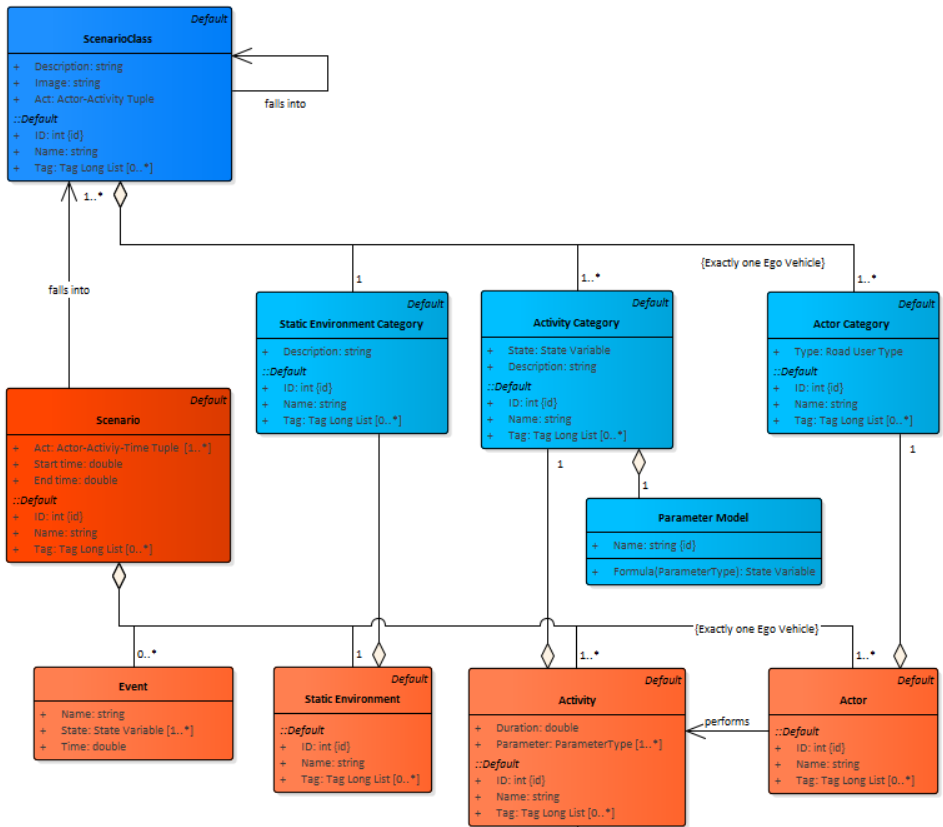
\includegraphics[width=\linewidth]{domain_model}
	\caption{Screen shot from Enterprise Architect with the domain model.}
	\label{fig:domain model}
\end{figure}

\subsubsection{Structure of the domain model}
\label{sec:structure domain model}

Because we want to differentiate between quantitative and qualitative descriptions, the definition of the term scenario is adopted from \cite{elrofai2018scenario} as it explicitly defines a scenario as a quantitative description: ``A scenario is a quantitative description of the ego vehicle, its activities and/or goals, its dynamic environment (consisting of traffic environment and conditions) and its static environment. From the perspective of the ego vehicle, a scenario contains all relevant events.'' Whereas a scenario refers to a quantitative description, these scenarios can be abstracted by means of a qualitative description, referred to as scenario class, see also \cite{ploeg2018cetran, elrofai2018scenario}. Scenario classes are formally described, see \cref{sec:qualitative scenario}. Next, we describe how scenarios are formally describes while making used of the classes defined for the formal description of scenario classes, see \cref{sec:quantitative scenario}.

To prevent duplications of some attributes, many classes are subclasses of the class \texttt{Default}. The class \texttt{Default} contains three attributes:
\begin{itemize}
	\item \texttt{id}: This is a unique identifier of type \texttt{Integer} that is used to refer to a specific object.
	\item \texttt{name}: This attribute is of type \texttt{String} and is used to help users understand what the object is about without looking for the details of the object. 
	\item \texttt{tag}: This attribute is a (possibly empty) list of \texttt{Tag}. Here, only a \texttt{Tag} can be chosen from a predefined enumeration.
	
	\color{red}
	TODO: Explain the function of tags.
	\color{black}
\end{itemize}
Note that \texttt{Default} is an abstract class, i.e., it is impossible to create instantiations of this class. It is, however, possible to create instantiations of subclasses.

\subsection{Qualitative description of scenario}
\label{sec:qualitative scenario}

As already mentioned in \cref{sec:structure domain model}, a scenario consists of a static environment and a dynamic environment. The dynamic environment consists of actors performing activities. Therefore, the classes \texttt{Actor}, \texttt{Activity}, and \texttt{StaticEnvironment} are used to define a scenario. Analogously, the classes \texttt{ActorCategory}, \texttt{ActivityCategory}, and \texttt{StaticEnvironmentCategory} are owned by \texttt{ScenarioClass}. We will first describe the classes \texttt{ActorCategory}, \texttt{ActivityCategory}, and \texttt{StaticEnvironmentCategory} before describe how a scenario class is defined.

To illustrate the use of the different classes, an example is presented. This example explains how a scenario can be qualitatively described where the ego vehicle is driving towards a vehicle that is driving at a lower speed. 

\subsubsection{The class \texttt{ActorCategory}}
\label{sec:actor category}

An object from the class \texttt{ActorCategory} describes an actor in qualitative terms. Here, an actor is an element of a scenario acting on its own behalf \cite{ulbrich2015}. In practice, this can be a driver of a car, a bicyclist, a pedestrian, an automation system, or a combination of a driver and an automation system \cite{geyer2014}. 

Next to the attributes that this class inherits from \texttt{Default}, it has attribute \texttt{type} which specifies the type of the actor, e.g., a vehicle or a pedestrian. The attribute \texttt{type} needs to be chosen from a predefined enumeration \texttt{RoadUserType}. 

For the future, it might be that we need to add a ``dynamic model'' that describes the dynamics of the actor. For now, we ignored this.

\begin{example}[Gap closing --- Actors] \label{example:actor category}
	In a scenario with an ego vehicle that drives towards a vehicle that is driving at a lower speed, two actors are defined. Hence, there need to be two objects from \texttt{ActorCategory}, see the following code.
	
	\begin{lstlisting}[caption=Code for instantiating two objects of \texttt{ActorCategory}.]
EGO_VEHICLE = ActorCategory(id = 1,
                            name = "Ego vehicle",
                            type = RoadUserType.Vehicle,
                            tags = [Tag.EgoVehicle])
TARGET_VEHICLE = ActorCategory(id = 2,
                               name = "Target vehicle",
                               type = RoadUserType.Vehicle,
                               tags = [Tag.InitState_LongPosition_InFrontOfEgo,
                                       Tag.InitState_Direction_SameAsEgo,
                                       Tag.InitState_LatPosition_SameLane])
	\end{lstlisting}
\end{example}

\subsubsection{The class \texttt{ActivityCategory}}
\label{sec:activity category}

An activity refers to the behavior of a particular mode. For example, an activity could be described by the label `braking' or `changing lane'. In each mode, the behavior of the system is described by a
particular model with a fixed function $f$, parameter $\theta$ and smooth input $u(t)$ \cite{deschutter2000optimal}. This model describes the state \cite{norman2011control}, where the state refers to ``[...] variables that define the characteristics of a system, component, or simulation'' according to the IEEE Standard Glossary of Software Engineering Terminology \cite{ieee1990glossary}. For example, a state could be the acceleration of an actor.

An object from the class \texttt{ActivityCategory} describes an activity in qualitative terms. Next to the attributes that this class inherits from \texttt{Default}, it has attributes \texttt{state} and \texttt{model} (note that \cref{fig:domain model} also shows the attribute \texttt{description}, but this attribute is not considered anymore). The attribute \texttt{state} needs to be chosen from a predefined enumeration \texttt{StateVariable}. The attribute \texttt{model} needs to be an object of the class \texttt{ParameterModel}.

Note that the actual parameters of the model are not defined, because this class describes the activity in qualitative terms. 

\begin{example}[Gap closing --- Activities] \label{example:activity category}
	We already saw that in a scenario with an ego vehicle that drives towards a vehicle that is driving at a lower speed, two actors are defined. We assume that both actors are driving forward and driving straight. Note that both vehicles drive with a different speed, so the activity that describes the longitudinal behavior is different for both actors. However, in qualitative terms, the activities are the same. Also for the lateral behavior, we only need one qualitative description. Hence, in total, we need to objects of \texttt{ActivityCategory}, see the following code. Note that for simplicity, it is assumed that the state can be described by a linear model, i.e., \texttt{Linear()}. Here, \texttt{Linear} is a subclass of \texttt{ParameterModel}. 
	
	\begin{lstlisting}[caption=Code for instantiating two objects of \texttt{ActivityCategory}.]
GOING_STRAIGHT = ActivityCategory(id = 1,
                                  name = "Going straight",
                                  model = Linear(), 
                                  state = StateVariable.LATERAL_POSITION,
                                  tags = [Tag.LatActivity_GoingStraight])
GOING_STRAIGHT = ActivityCategory(id = 2,
                                  name = "Going forward",
                                  model = Linear(), 
                                  state = StateVariable.LONGITUDINAL_POSITION,
                                  tags = [Tag.LongActivity_DrivingForward])
	\end{lstlisting}
\end{example}

\subsubsection{The class \texttt{StaticEnvironmentCategory}}
\label{sec:static environment category}

An object from the class \texttt{StaticEnvironmentCategory} describes the static environment in qualitative terms. The static environment refers to the part of a scenario that does not change during a scenario. This includes geo-spatially stationary elements \cite{ulbrich2015}.

Next to the attributes that this class inherits from \texttt{Default}, it has attribute \texttt{description} of type \texttt{String} which enables the user to provide more details about the static environment.

\begin{example}[Gap closing --- Static environment] \label{example:static environment category}
	For this scenario class, we do not want to describe anything about the static environment. In other words, a scenario that falls into this scenario class can happen on, e.g., a highway, an urban road, or a junction. Therefore, no additional tags are defined. The following code illustrates how such a static environment can be defined.
	
	\begin{lstlisting}[caption=Code for instantiating an object of \texttt{StaticEnvironmentCategory}.]
STATIC_DESC = "No further details are specified for the static environment."
STATIC_ENVIRONMENT = StaticEnvironmentCategory(id = 1,
                                               name = "Anything",
                                               description = STATIC_DESC,
                                               tags = [])
	\end{lstlisting}
\end{example}

\subsubsection{The class \texttt{ScenarioClass}}
\label{sec:scenario class}

Next to the attributes that this class inherits from \texttt{Default}, \texttt{ScenarioClass} has the following attributes:
\begin{itemize}
	\item \texttt{description}: This is a text of type \texttt{String} that enables the user to provide more details about the scenario class.
	\item \texttt{image}: This enables the user to define a path to an image that (schematically) shows the scenario class. This attribute is of type \texttt{String}.
	\item \texttt{actors}: This attribute is a list containing objects of type \texttt{ActorCategory} as described in \cref{sec:actor category}. This list needs to contain at least one \texttt{ActorCategory}.
	\item \texttt{activities}: This attribute is a list containing objects of type \texttt{ActivityCategory} as described in \cref{sec:activity category}. This list needs to contain at least one \texttt{ActivityCategory}.
	\item \texttt{static\_environment}: This attribute describes the static environment in which the scenario happens. This attribute is of type \texttt{StaticEnvironmentCategory} as described in \cref{sec:static environment category}.
	\item \texttt{act}: This attribute is a list of tuples, with each tuple containing one \texttt{ActorCategory} and one \texttt{ActivityCategory}. These acts connect the activities with the actors. 
\end{itemize}

\begin{example}[Gap closing --- Scenario class]
	To define the scenario class gap closing, use is made of the previously defined objects, i.e., the \texttt{EGO\_VEHICLE} and \texttt{TARGET\_VEHICLE} from \cref{example:actor category}, \texttt{GOING\_STRAIGHT} and \texttt{GOING\_FORWARD} from \cref{example:activity category}, and \texttt{STATIC\_ENVIRONMENT} from \cref{example:static environment category}.
	
	\begin{lstlisting}[caption=Code for instantiating an object of \texttt{ScenarioClass}.]
SC_NAME = "Ego vehicle approaching slower lead vehicle"
SC_DESC = "Another vehicle is driving in front of the ego vehicle at a " + \
          "slower speed. As a result, the other vehicle appears in the " + \
          "ego vehicle's field of view. The reason for the other vehicle " + \
          "to drive slower is, e.g., due to a traffic jam ahead."
SC_IMAGE = "gap_closing.png"
GAP_CLOSING = ScenarioClass(id = 1,
                            name = SC_NAME,
                            description = SC_DESC,
                            actors = [EGO_VEHICLE, TARGET_VEHICLE],
                            activities = [GOING_STRAIGHT, GOING_FORWARD],
                            static_environment = STATIC_ENVIRONMENT,
                            acts = [(EGO_VEHICLE, GOING_STRAIGHT),
                                    (EGO_VEHICLE, GOING_FORWARD),
                                    (TARGET_VEHICLE, GOING_STRAIGHT),
                                    (TARGET_VEHICLE, GOING_FORWARD)])
	\end{lstlisting}
\end{example}

\subsection{Quantitative description of scenario}
\label{sec:quantitative scenario}

\color{red}
TODO: The classes that are used to quantitatively describe a scenario (i.e., \texttt{Scenario}, \texttt{Event}, \texttt{StaticEnvironment}, \texttt{Activity}, and \texttt{Actor}) need to be described.
\color{black}.

\cbend
\printbibliography

\end{document} 